%\setchapterimage{fig_00.jpg}
\chapter*{TD \arabic{cptApplication} \\ 
Machine de forage -- \ifprof Corrigé \else Sujet \fi}
\addcontentsline{toc}{section}{TD \arabic{cptApplication} : Machine de forage -- \ifprof Corrigé \else Sujet \fi}

\iflivret \stepcounter{cptApplication} \else
\ifprof  \stepcounter{cptApplication} \else \fi
\fi

\setcounter{question}{0}
\marginnote{D'après Concours CCINP 2023 -- MP.}
\marginnote[1cm]{
\UPSTIcompetence[2]{B2-14}
\UPSTIcompetence[2]{C1-05}
\UPSTIcompetence[2]{C2-07}
}

\begin{marginfigure}
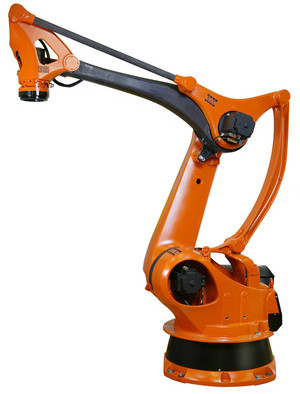
\includegraphics[width=\linewidth]{fig_01}
\end{marginfigure}


Dans le domaine du génie civil, les foreuses permettent de réaliser des perçages profonds afin de couler des pieux en béton armé. On s'intéresse aux conditions de basculent statique de la foreuse. 


\begin{figure}[!h]
\centering
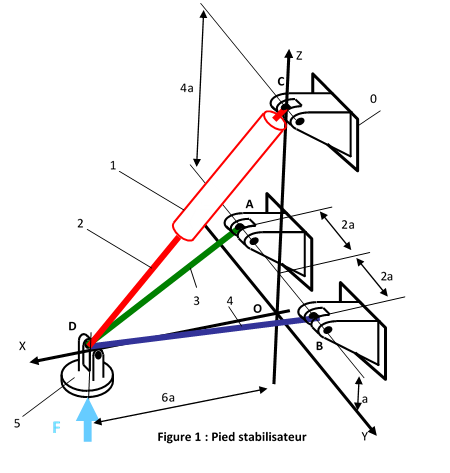
\includegraphics[width=.8\linewidth]{fig_02}
\caption{Paramétrage mécanique}
\end{figure}

Soient : 
\begin{itemize}
\item \textbf{0} le sol, \textbf{S1} le châssis de la foreuse, \textbf{S2} sa tourelle et son mât et \textbf{S3} l’ensemble \{table de forage + outil\} ; 
\item $\rep{0} = \repere{O}{x}{y}{z}$ le repère attaché aux solides \textbf{S0} et \textbf{S1}; 
\item $\mathcal{B}_2=\base{x_2}{y_2}{z_2}$ la base attachée aux solides \textbf{Sé} et \textbf{S3} telle que $\angl{x}{x_2}=\theta$ où $\theta$ est connu ;
\item $\Sigma = $ \textbf{\{S1, S2, S3\}} l’ensemble de la foreuse, de centre de gravité $G$ tel que $\vect{OG} = r \vx{2} +  z_G \vect{z}$;
\item $M = \SI{186,5}{tonnes}$ la masse de l’ensemble $\Sigma$ et $m =\SI{18}{tonnes}$ la masse de \textbf{S3} seul ; 
\item $2F_w \vect{z}$ connu, l’effort du câble d’avance sur \textbf{S3}. La masse du câble est négligée dans la suite ; 
\item $\indice{F}{sol}\vect{z}$, inconnu, l’effort de forage du sol \textbf{0} sur l’outil de forage \textbf{S3} au point $F$, connu, défini par $\vect{OF}=R\vx{2}$;
\item $-g\vect{z}$  où $g = \SI{9,8}{m.s^{-2}}$, l’accélération de la pesanteur terrestre.
\end{itemize}

On modélise ici les contacts entre le sol et la foreuse\textbf{par des contacts ponctuels}  :
$F_g \vect{z}$, (respectivement  $F_d \vect{z}$) inconnu, l’effort du sol 0 sur S1, supposé ponctuel au centre $I$ (respectivement  $J$) de la surface de contact entre la chenille gauche $cg$ (respectivement  $c_d$) et le sol tel que $||\vect{OI}|| = a=\SI{2,1}{m}$ (respectivement  $||\vect{OJ}|| = a=\SI{2,1}{m}$).

